
\subsection{The Average Causal Response (ACR) Framework}
\label{section:acr-detail}

More formally, let $ N_{0i} $ and $ N_{1i} $ be the potential number of children in the family if a binary instrument $ Z_{i} $ were equal to 0 and 1, respectively. The observed number of children $ n_{i} $ is then, $ n_{i} = N_{0i} + (N_{1i} - N_{0i})\cdot Z_{i} $. Similarly let $ Y_{i}(j) $ be the potential outcome as a function of $ j $, where j takes possible values for $ n_{i} $ in the set $ \{0, 1, \dots, J\} $. Only one of these potential outcomes is realized and we denote the observed outcome by $ y_{i} $. In the simplest case with no covariates, the IV estimator using a binary instrument $ Z $ gives the Wald estimator.\footnote{The interpretation of the ACR is more elaborate when covariates are added, but the basic idea is preserved. See \textcite[p.~437]{Angrist1995}.} Then,


\begin{equation}\label{eq:02}
	\beta_{w} = \dfrac{\mathbb{E}(y_{i} | Z_{i} = 1) - \mathbb{E}(y_{i} | Z_{i} = 0)}{\mathbb{E}(n_{i} | Z_{i} = 1) - \mathbb{E}(n_{i} | Z_{i} = 0)} = \sum_{j = 1}^{J} \omega_{j}\cdot \mathbb{E}(Y_{i}(j) - Y_{i}(j-1) | N_{1i} \geq j > N_{0i})
\end{equation}

where
\begin{equation}\label{eq:03}
\omega_{j} = \dfrac{\mathbb{P}(N_{1i} \geq j > N_{0i})}{\sum_{i = 1}^{J} \mathbb{P}(N_{1i} \geq i > N_{0i})}
\end{equation}
\vskip10pt

The unit causal response in \eqref{eq:02}, $ \mathbb{E}(Y_{i}(j) - Y_{i}(j-1) | N_{1i} \geq j > N_{0i}) $, is the average difference in potential outcomes for \textit{compliers} at point $ j $; that is, individuals driven by the instrument from a treatment intensity less than $ j $ to at least $ j $.\footnote{We are using the word \enquote{compliers} in the context of the treatment-effects framework outlined in \textcite{angrist_identification_1996}. See the discussion below for more explanation.} Thus, the Wald estimator, $ \beta_{w} $, is \enquote{a weighted ACR for people from families induced by an instrument to go from having fewer than $ j $ to at least $ j $ children, weighted over $ j $ by the probability of crossing this threshold} \parencite[p.~787]{angrist_multiple_2010}. The numerator in the expression for the weights $ \omega_{j} $ in \eqref{eq:03}, $ \mathbb{P}(N_{1i} \geq j > N_{0i}) $, represents the proportion of compliers at point $ j $.\footnote{Individuals with $ N_{1i} \geq j > N_{0i} $  for any $ j $ in the support of $ n_{i} $ are considered as compliers.} This is normalized by $ \sum_{i = 1}^{J} \mathbb{P}(N_{1i} \geq i > N_{0i}) $, which can be shown to be equal to the Wald first stage \parencite[see][p.~183]{Angrist2009}. That is,

\begin{equation}\label{eq:04}
\mathbb{E}(n_{i} | Z_{i} = 1) - \mathbb{E}(n_{i} | Z_{i} = 0) = \sum_{i = 1}^{J} \mathbb{P}(N_{1i} \geq i > N_{0i})
\end{equation}

There are three assumptions that lie behind the ACR theorem: (i) independence and exclusion; (ii) the existence of a first Stage; and (iii) monotonicity \parencite{Angrist2009}. The independence assumption requires that the instrument be independent of potential outcomes and potential treatment assignments. This is sometimes alternatively stated by saying that the instrument need to be as good as randomly assigned. Both the twins and same sex instruments were originally proposed as natural experiments for fertility on the ground that both are virtually randomly assigned \parencite{rosenzweig_testing_1980,angrist_children_1998}. However, this is no longer obvious because various threats to the randomness of both instruments have been pointed out in the literature (see Section~\ref{section:valid}). The exclusion assumption, on the other hand, says that the instrument used has no effect on the outcomes other than through its effect on family size.  Although this is closely related to the independence assumption, it is distinct from it. The exclusion restriction is a \enquote{a claim about a unique channel for causal effects of the instrument} \parencite[p.~153]{Angrist2009}. Again, various authors have pointed out ways in which exclusion restriction might fail to hold for both instruments. I have tried to address some of the important concerns in Section~\ref{section:valid}.\footnote{ The other important assumption needed to estimate the ACR is monotonicity. In our case, monotonicity requires that the proposed instrument moves fertility in one direction only. In particular, we assume that the potential number of children when the instrument is switched on is at least as large as it would have been when it is switched off; i.e., $ N_{1i} \geq N_{0i} $. This is automatically satisfied by the twins instrument as fertility is always increased because of a twin birth for any mother. Although rare, it is possible that monotonocity might fail to hold for the same sex instrument. For example, there could be parents who prefer children of the same sex and therefore go on to have another child if the sexes of the first two or three children are different \parencite{Huber2015}. As a partial check on monotonicity, I estimated the same sex first stage in the 2+ sample for each combination of the mother's population group, intervals of the mother's age at first birth, and the level of education of the mother. Out of the 44 first stage regressions, corresponding to the 44 cells, only three generate negative estimates and all three were insignificant. The remaining significant estimates were all positive.} 

%The other important assumption needed to estimate the ACR is monotonicity. To understand the idea behind this assumption, we need to introduce the four mutually exclusive groups comprising of our quasi-experimental population: compliers, always takers, never takers, and defiers. These were first outlined in the treatment-effects framework of \textcite{angrist_identification_1996}.  Always takers always get treated regardless of their assignment, never takers never get treated regardless of their assignment, and compliers get treated when the instrument is switched on and don't get treated otherwise. The defiers, on the other hand, are a very strange group who get treated when the instrument is switched off and don't get treated when it is switched on. The assumption of monotonicity rules out the presence of defiers since they complicate the link between ACR and the reduced form \parencite{Angrist2009}.\footnote{\textcite{Angrist2009} discuss monotonicity in the context of the LATE framework of \textcite{imbens_identification_1994}. But this carries over directly to the ACR since the ACR is just an extension of the LATE \parencite[see][p.~181]{Angrist2009}.}  In other words, monotonicity rules out the case where the instrument pushes some people into treatment while pushing others out. In our case, monotonicity requires that the proposed instrument moves fertility in one direction only. In particular, we assume that the potential number of children when the instrument is switched on is at least as large as it would have been when it is switched off; i.e., $ N_{1i} \geq N_{0i} $. This is automatically satisfied by the twins instrument as fertility is always increased because of a twin birth for any mother. However, monotonicity need not hold for the same sex instrument as there could be parents who prefer children of the same sex and therefore go on to have another child if the sexes of the first two or three children are different \parencite{Huber2015}. In Section~\ref{section:samesx}, I discuss a partial check for monotonicity using first stage regressions. 

\pagebreak

\begin{figure}[ht]
\centering
\caption{\label{fig:02}Unconditional First-Stages and 95\% Confidence Intervals for Different Family Sizes}
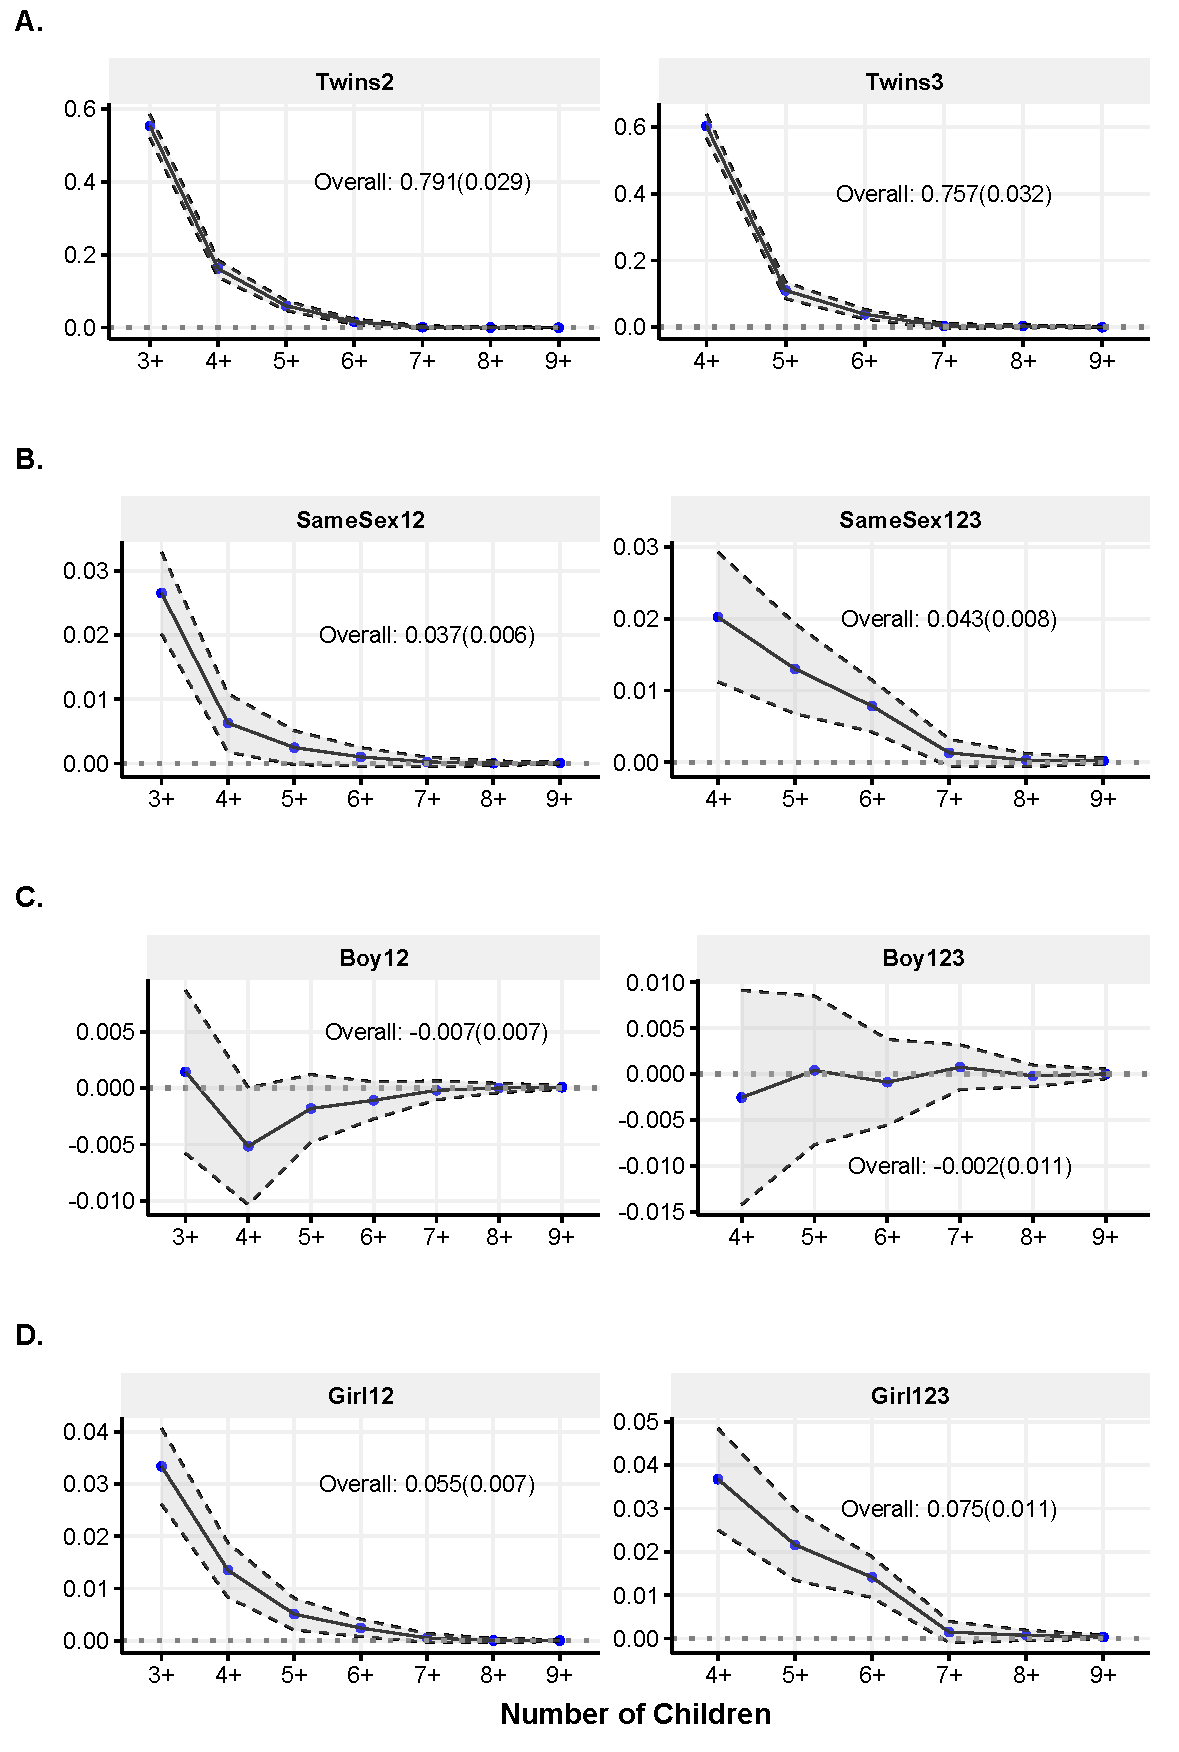
\includegraphics[width=\textwidth]{figures/acrs.pdf}
% This could go to the addendum
\end{figure}

\begin{figure}[p!]
\centering
\caption{\label{fig:heter1}Results of Generalized Random Forest Using Twins IV}
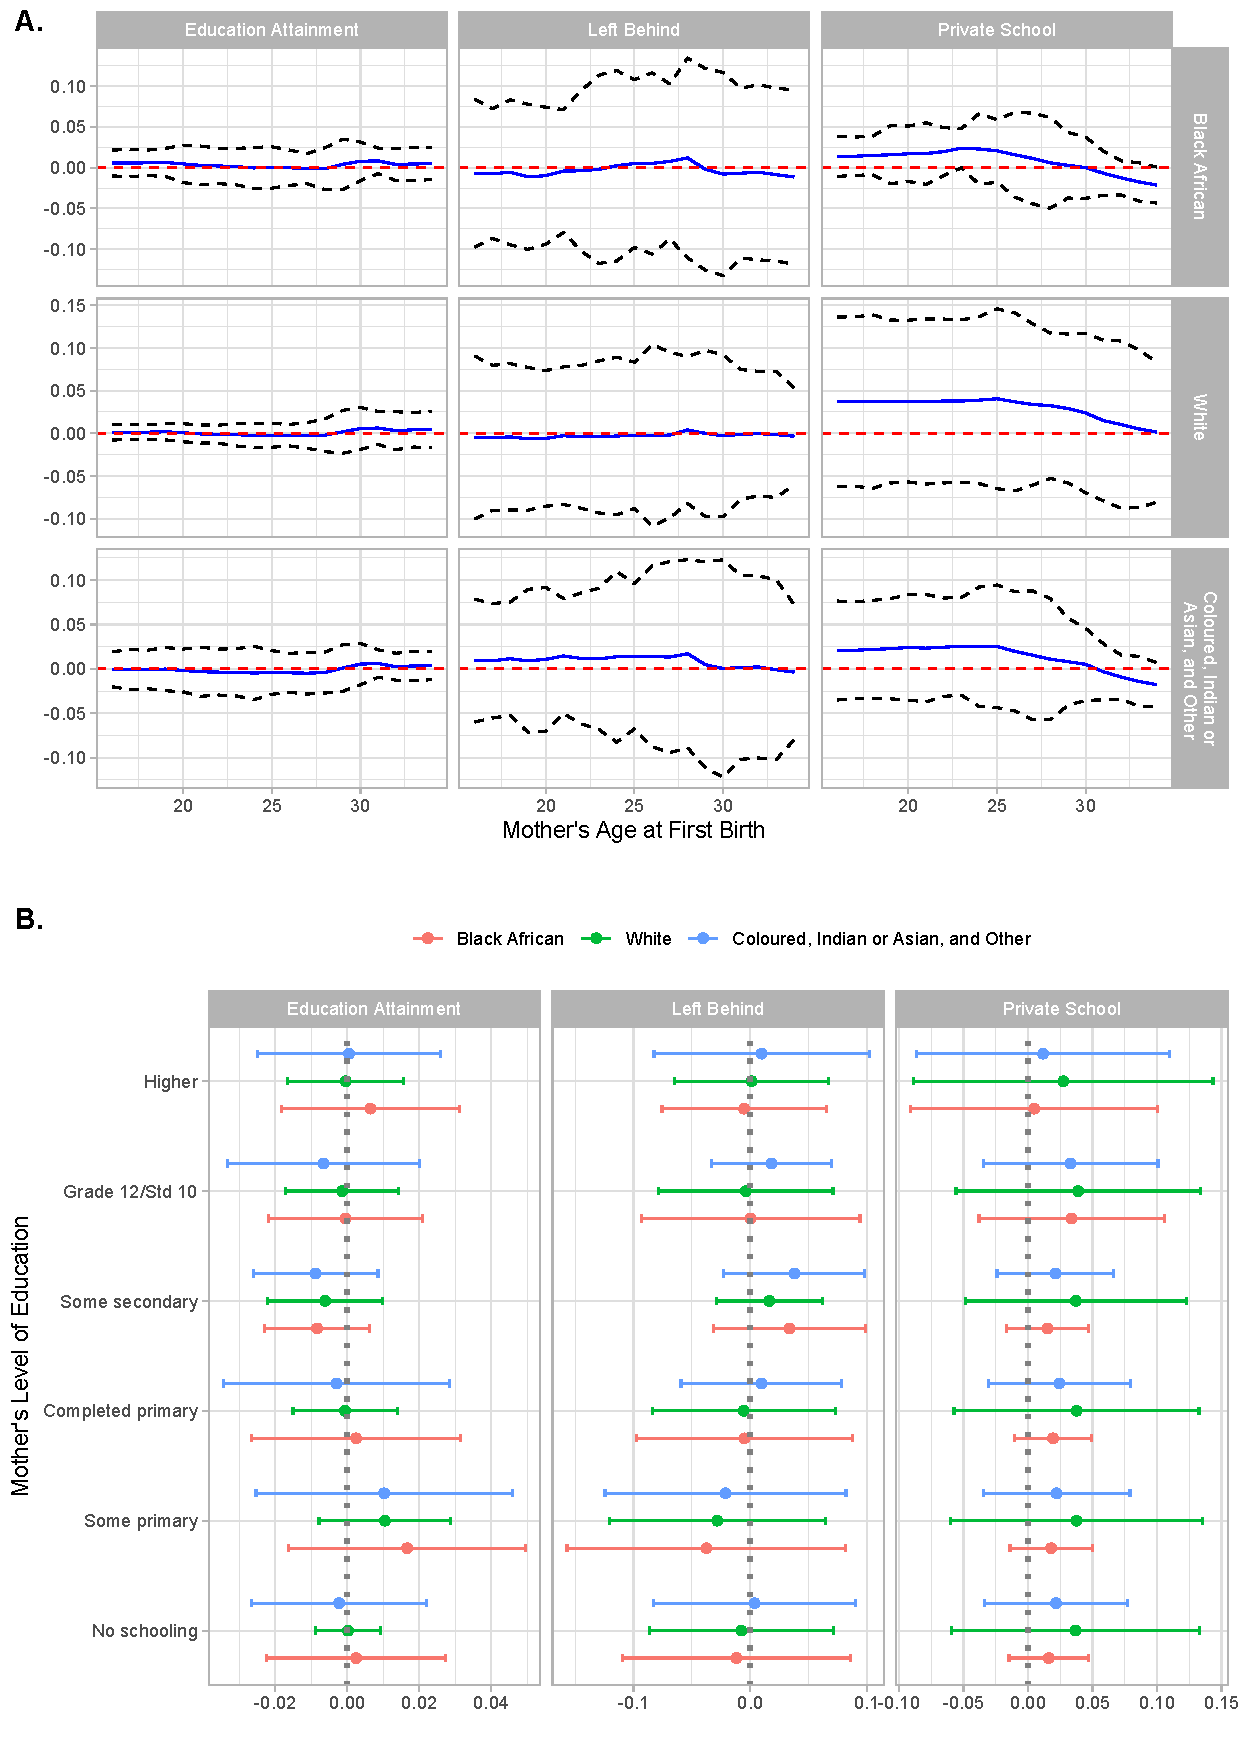
\includegraphics[width=\textwidth]{figures/heter1.pdf}
\fnote{\textit{Notes:} The above results are based on three forests, one forest for each outcome. Tuning results suggest the default values of the parameters as optimal for each forest: subsample fraction ($ s/n $) $ = 0.5 $, minimum leaf size ($ k $) $ = 5 $, number of splitting variables (\texttt{mtry}) $ = 26 $ (out of 33), balance parameter ($ \alpha $) $ = 0.05 $, and imbalance penalty $ = 0 $ (see the software implementation of \textcite{Athey2019} for the description of these parameters). Each forest is based on 5000 trees.}
\end{figure}
\pagebreak

\begin{figure}[p!]
\centering
\caption{\label{fig:heter2}Results of Generalized Random Forest Using Same-Sex IV}
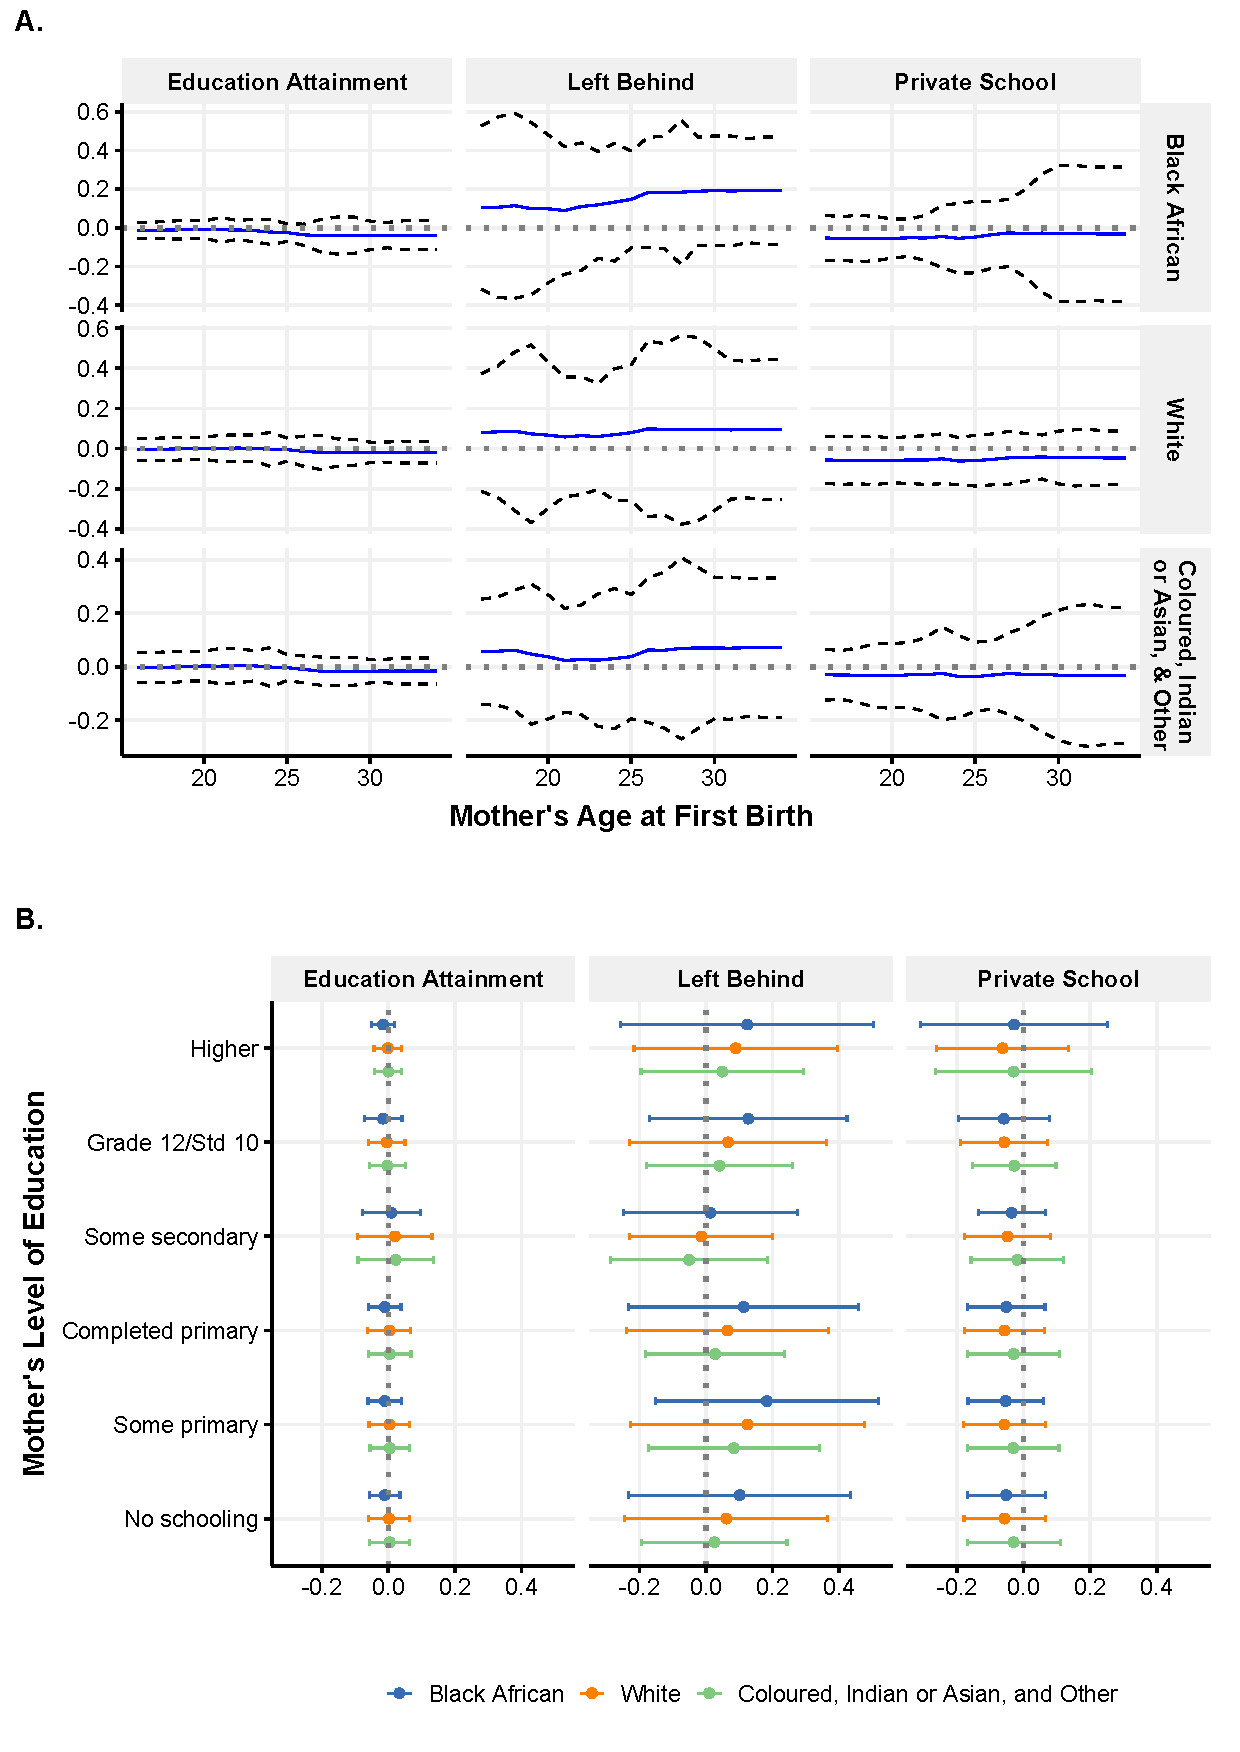
\includegraphics[width=\textwidth]{figures/heter2.pdf}
\fnote{\textit{Notes:} The above results are based on three forests, one forest for each outcome. The parameters supplied in training each forest were chosen by tuning based on cross-validation and are shown in the table below:
\centering
\begin{tabular}{rrrrrr}
  \hline
 & sample.fraction & mtry & min.node.size & alpha & imbalance.penalty \\ 
  \hline
educ & 0.25 & 7.00 & 53.00 & 0.21 & 0.55 \\ 
  behind & 0.08 & 8.00 & 71.00 & 0.07 & 1.26 \\ 
  private & 0.10 & 9.00 & 83.00 & 0.10 & 3.12 \\ 
   \hline
\end{tabular}
  Each forest is based on 5000 trees. }
\end{figure}
\pagebreak
